\chapter{Physics-Informed Transient Characterisation and Modelling of IBRs} \label{ch_2}

Protection challenges are introduced because the output current of an IBR facility is very different from a traditional rotating synchronous source facility during short circuit conditions. This chapter presents the transient characterisation and modelling of IBRs to understand the fault current composition and grid code–driven responses during network fault events.

\section{Fundamentals of Converter-Interfaced Dynamics: Transition from Inertial to Low-Inertia Systems}
In legacy architectures, frequency stability is predicated on the inherent kinetic energy ($E_{kin} = \frac{1}{2} J \omega^2$) stored in the rotating masses of synchronous machines, which serves as an autonomous physical buffer. Conversely, IBRs effectively decouple the primary energy source from the network frequency, resulting in a system where stability is no longer governed by laws for rotation, but by the bandwidth of power-electronic control loops. This decoupling manifests as a significant increase in the Rate of Change of Frequency (RoCoF), where the frequency nadir is reached within milliseconds rather than seconds.
% Protection challenges are introduced because the output current of an IBR facility is very different from a traditional rotating synchronous source facility during short circuit conditions. Current from a synchronous source, immediately after a short circuit and within the timeframe of protection operation, is of high magnitude, uncontrolled and can be mostly defined by electrical parameters of the source and impedance of short circuit path. 
% However, the short circuit current of the IBR is of low magnitude, highly controlled and managed by using fast switching of power electronics devices dependent upon manufacturer-specific and often proprietary control system design. One of the key control design objectives is limiting the magnitude of current within the thermal withstand capability of power electronics during short circuits while meeting the grid code requirements (if applicable). Thus, an IBR has low-magnitude and non-universal short circuit current characteristic.In addition, weather conditions introduce large changes in IBR output and that may have a negative influence on line protection reliability. Not taking into account the differing nature of IBR behavior, traditional line protection may incorrectly trip for some external short circuits or may not trip on other internal short circuits.

% The rapid proliferation of Inverter-Based Resources (IBRs)—including photovoltaic (PV) and wind energy conversion systems—has transformed the operational behavior of modern electric power systems. Unlike conventional synchronous machines that provide high-magnitude fault currents, IBRs employ power electronic converters that tightly control current amplitude and phase during faults. Consequently, their short-circuit response deviates fundamentally from classical electromechanical dynamics, leading to inaccurate fault level estimation, misoperation of relays, and reduced protection sensitivity.





\section{Mathematical Characterization of Solar PV Systems: DC-Link Dynamics and V-I Characteristic Curves}

\begin{figure*}[!h]
\centering
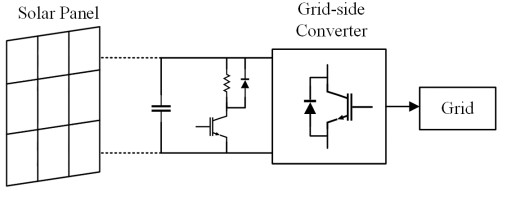
\includegraphics[scale=0.8]{images/chapter_2/Ch2F1Jul.jpg}
\caption{Basic configuration of solar photovoltaic (PV) energy conversion source}
\label{VPP sim}
\end{figure*}
The transient response of a grid-tied PV system is fundamentally anchored to the non-linear V-I characteristic of the semiconductor-based source. Unlike a synchronous machine, which behaves as a voltage source behind a sub-transient reactance, a PV array is a current-limited non-linear device. The output current $I_{pv}$ is defined by the transcendental diode equation:

\begin{equation}
\label{eq:vtdq}
I_{pv} = I_{ph} - I_{o} \left[ e^{\frac{q(V_{pv} + I_{pv}R_s)}{nkT}} - 1 \right] - \frac{V_{pv} + I_{pv}R_s}{R_{sh}}
\end{equation}

% $$I_{pv} = I_{ph} - I_{o} \left[ e^{\frac{q(V_{pv} + I_{pv}R_s)}{nkT}} - 1 \right] - \frac{V_{pv} + I_{pv}R_s}{R_{sh}}\text{ [\cite{li2025gridforming}]}$$

This establishes the source as fundamentally current-limited before the conversion stage, possessing a specific Maximum Power Point (MPP) defined by the coordinates ($V_{mpp}, I_{mpp}$).

\subsubsection{DC-Link Stability and Energy Balance}
DC-link stability is governed by the instantaneous energy balance between the PV harvesting stage and the grid-side conversion stage. The governing differential equation for the DC-link voltage $V_{dc}$ is:

\begin{equation}
\label{eq:vtdq}
C_{dc}\frac{dV_{dc}}{dt} = I_{pv} - I_{conv} = \frac{P_{pv}}{V_{dc}} - \frac{P_{grid}}{V_{dc}} 
\end{equation}


$I_{conv}$: The current drawn by the inverter to satisfy grid demands.
\\
This equation links the DC-side energy storage directly to the AC-side power flow, making $V_{dc}$ a critical indicator of system stability

\subsubsection{Fault-Induced Power Mismatch}

During an asymmetrical AC fault, the reduction in grid voltage ($V_{dq}$) creates a power mismatch that manifests as a DC-link voltage excursion. Considering the grid power equations:

\begin{equation}
\label{eq:vtdq}
P_{grid} = \frac{3}{2}V_d I_d
\end{equation}

If $V_d$ drops due to a fault while $P_{pv}$ remains constant (driven by the MPPT loop), the resulting term $\frac{dV_{dc}}{dt} > 0$ leads to rapid capacitor overcharge.
\\
To protect the DC-link capacitor and inverter bridge from catastrophic overvoltage, the control software must intervene to clamp the current and redirect or curtail power.





\subsection{The "Software-Defined" Fault Current: MPPT vs. Fault Ride-Through (FRT) Conflict}

The "Software-Defined" nature of the fault current in modern Inverter-Based Resources (IBRs) arises from the intense algorithmic competition between the Maximum Power Point Tracking (MPPT) loop and the Fault Ride-Through (FRT) supervisor. Unlike synchronous machines, where the fault response is an autonomous physical reaction of the magnetic circuit, an IBR's response is a purely mathematical trade-off between active and reactive power references.


\subsubsection{The Algorithmic Competition}
Under steady-state conditions, the inverter control system operates in an MPPT-dominant mode, seeking to satisfy the condition:

\begin{equation}
\label{eq:vtdq}
\frac{dP_{pv}}{dV_{pv}} = 0
\end{equation}

Simultaneously, to maintain grid stability during disturbances, modern grid codes (e.g., IEEE 1547-2018) mandate the injection of dynamic reactive current ($I_q$) proportional to the voltage deviation:

\begin{equation}
\label{eq:vtdq}
I_q = K_q(V_{ref} - V_{pcc}) 
\end{equation}


The inherent conflict arises because $I_q$ priority fundamentally reduces the available $I_d$ capacity for power export. This necessitates a transition from power-harvesting logic to a protective "clamping" state.

\subsubsection{Forced Curtailment and "Clamped" Signatures}
Under deep voltage sags, the controller must prioritize reactive support ($I_q$), leading to the forced curtailment of active power ($P$). Because the inverter is limited by its semiconductor thermal rating ($I_{max}$), the maximum allowable active current reference ($I_{d,max}$) is restricted by the following orthogonal constraint:
\begin{equation}
\label{eq:vtdq}
I_{d,max} = \sqrt{I_{max}^2 - I_{q,ref}^2}
\end{equation}
This creates a "clamped" current signature where the phase angle ($\phi$) is no longer a function of the fault impedance, but is purely a function of the internal control logic:
\begin{equation}
\label{eq:vtdq}
\phi = \tan^{-1}\left(\frac{I_q}{I_d}\right)
\end{equation}

This "Software-Defined" phase angle effectively blinds legacy directional elements (ANSI 67), as the voltage-current relationship is dictated by the $K_q$ slope rather than the physical $X/R$ ratio of the faulted circuit.

\subsubsection{Transient Signature Characterization}
The resulting transient signature is characterized by a brief, sub-cycle discharge of filtering components followed by a static, symmetric current profile held by the software. The instantaneous fault current $i(t)$ can be modeled as:
\begin{equation}
\label{eq:vtdq}
i(t) = I_{max} \sin(\omega t + \phi_{control}) + i_{transient}(e^{-t/\tau}) 
\end{equation}

Sub-cycle Transient ($i_{transient}$): The brief sub-cycle discharge is primarily due to the sudden energy release from AC filter capacitors and DC-link dynamics.Steady-State Regulated Source 
\\
($I_{fault}$): Following the initial transient, the output becomes a regulated current source:

\begin{equation}
\label{eq:vtdq}
I_{fault} = I_{max} e^{j\phi_c}
\end{equation}

This "clamping" behavior justifies the failure of conventional inverse-time overcurrent relays (ANSI 51). Because the current does not "jump" to high levels but is strictly "held" by the software, the relay's operating time exceeds the critical clearing time, or the fault remains entirely undetected within the relay's deterministic pickup thresholds.

\section{Transient Response of Wind Turbine Generators (WTGs)}


\begin{figure*}[!h]
\centering
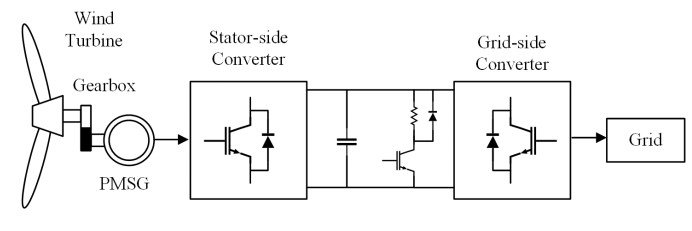
\includegraphics[scale=0.7]{images/chapter_2/Ch2F2Jul.jpg}
\caption{Basic configuration of Type IV wind energy conversion source}
\label{VPP sim}
\end{figure*}

\begin{figure*}[!h]
\centering
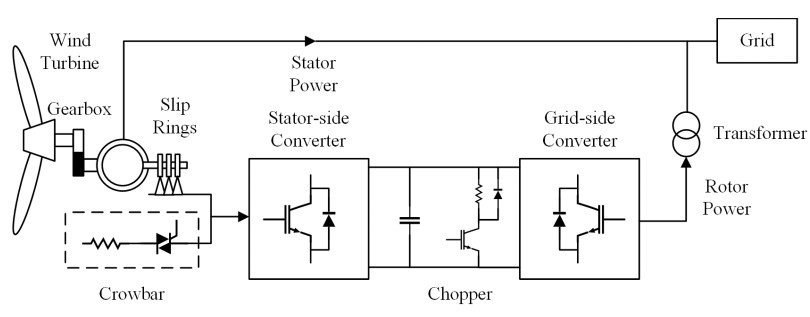
\includegraphics[scale=0.7]{images/chapter_2/Ch2F3Jul.jpg}
\caption{Basic configuration of Type III wind energy conversion source}
\label{VPP sim}
\end{figure*}

\subsection{Type III (DFIG) Crowbar Dynamics}
he transient response of a Doubly-Fed Induction Generator (DFIG) is characterized by a dual-stage transition. Under normal operation, the rotor-side converter (RSC) maintains independent control of active and reactive power. However, severe grid voltage sags induce high electromotive forces (EMF) in the rotor windings, threatening the RSC's semiconductor integrity.
\subsubsection{Stage 1: The Induction Generator Transition}
To protect the RSC, a "crowbar" circuit (a set of resistors connected via thyristors) is activated, short-circuiting the rotor windings. This effectively transforms the DFIG from a controlled current source into a conventional squirrel-cage induction generator (SCIG). The short-circuit current $i_{sc}(t)$ during this period is governed by:
\begin{equation}
i_{sc}(t) = \frac{V_s}{X'_{s}} \left[ e^{-t/T'_s} - (1-\sigma)e^{-t/T'_r} e^{j\omega_r t} \right] 
\end{equation}

Where:\\
$V_s$: Stator terminal voltage.\\
$X'_s$: Stator transient reactance.\\
$T'_s, T'_r$: Stator and rotor transient time constants.\\
$\sigma$: Leakage coefficient.

\subsubsection{Stage 2: Deterministic Failure}
The activation of the crowbar consumes significant reactive power from the grid to maintain magnetization, further depressing the local voltage. This erratic, non-linear jump in current magnitude and phase angle is fundamentally untrackable by legacy distance relays (ANSI 21), as the apparent impedance ($Z_{app}$) enters the trip zone in a non-deterministic trajectory.

\subsection{Type IV (Full-Converter) Signature Analysis}
Unlike Type III, the Type IV WTG is completely decoupled from the grid via a full-scale back-to-back converter. The transient signature is 100\% "Software-Defined" and governed by the current-limiting algorithms of the grid-side converter (GSC).

The GSC regulates the output current within a strict d-q frame, prioritizing reactive current ($I_q$) injection for grid support as mandated by IEEE 2800. The total fault current is strictly capped by the converter's thermal ceiling ($I_{max}$):

\begin{equation}
|I_{fault}| = \sqrt{I_{d,ref}^2 + I_{q,ref}^2} \leq I_{max} 
\end{equation}
Typically, $I_{max}$ is restricted to $1.1\text{--}1.3 \text{ p.u.}$. The phase angle of the injected current is dictated by:
\begin{equation}
\phi_{fault} = \tan^{-1}\left(\frac{I_{q,ref}}{I_{d,ref}}\right) 
\end{equation}

Because $I_{fault}$ is clamped to a near-rated symmetric profile within $10\text{--}20 \ ms$, legacy overcurrent relays (ANSI 51) fail to pick up. Furthermore, the artificial suppression of negative-sequence current ($I_2 \approx 0$) by the GSC control loops renders negative-sequence directional elements (ANSI 67Q) completely inoperative.





% Requires: \usepackage{array}
\begin{table}[h]
    \centering
    \begin{tabular}{|>{\raggedright\arraybackslash}p{5cm}|>{\raggedright\arraybackslash}p{10cm}|}
        \hline
        \textbf{Standard / Grid Code} & \textbf{Key Requirements} \\ \hline
        IEEE 1547-2018 / 1547a-2020 & DERs must ride through voltage/frequency disturbances (e.g., 0.5 pu voltage for 0.16–0.33 s). Momentary cessation allowed but tripping only outside defined time ranges. Dynamic voltage support is optional. \\ \hline
        IEEE 2800-2022 & Applies to transmission-connected IBRs. Requires fault ride-through (FRT) with reactive and negative-sequence current injection during faults. \\ \hline
        IEC 62786 Series & Global technical specification for DER FRT. Requires undervoltage ride-through (UVRT) and coordinates with IEC test standards. Modular parts cover different DER technologies and align with IEEE 1547 and European ENTSO-E codes. \\ \hline
        IEC 61850 (esp. 7-420, 90-7) & Communication standard enabling DER status/control (e.g., ride-through mode, current limits). Allows SCADA and relays to send or receive fault commands via GOOSE. \\ \hline
        Grid Codes (e.g., ENTSO-E, Germany) & Require DERs to stay online and inject reactive/negative-sequence current during faults. Often define detailed current-voltage ride-through curves. \\ \hline
        UL 1741 SB (USA) & Tests DERs for IEEE 1547 compliance. Inverters must pass FRT, voltage trip, and current injection behavior checks. \\ \hline
        NERC PRC-024 & Ensures large generators meet voltage/frequency ride-through criteria. Now mostly embedded in IEEE 2800. \\ \hline
    \end{tabular}
    \caption{Summary of Standards and Grid Codes with Key Requirements}
    \label{tab:standards-key-requirements}
\end{table}



%%%%%%%%%%%%%%%%%%%%%%%%%%%%%%%%%%%%%%%%%%%
% Grid-tied PV inverters are modeled as controlled current sources synchronized via PLLs. Their dq-axis current references are generated by:

% % dq-axis current control references
% \begin{equation}
% \label{eq:idqref}
% \begin{aligned}
% I_d^* &= \frac{2P^*}{3V_d} \\
% I_q^* &= -\frac{2Q^*}{3V_d}
% \end{aligned}
% \end{equation}

% During faults, control logic switches to LVRT mode, injecting reactive current proportional to the voltage sag. Thus, PV fault current models must include:

% DC-link capacitor dynamics, Current limiter saturation, and Control delay effects.

% % Inverter current limiting magnitude
% \begin{equation}
% \label{eq:ilim}
% |\mathbf{I}| = \sqrt{I_d^{*2} + I_q^{*2}} \leq I_{max}
% \end{equation}


% Figure 2.1 and Figure 2.2 illustrate basic configurations of solar and Type IV wind conversion resources, respectively. They have a full power electronic converter interface between the grid and the resource. The interface is sized based on the total power output of the generation. Type III wind energy conversion resource is a doubly fed asynchronous generator whose stator directly connects to the grid and the rotor through a power electronic converter as shown in Figure 2.3. In this case, the interface is sized based on a fraction (about 30\%) of the total generation capacity. All three types of resources are referred to as inverter-based resource (IBR) for convenience. 

% IBRs are categorized based on their converter interfaces and control topologies. The short-circuit model depends on the nature of the fault, converter rating, grid coupling, and applied control strategies. During faults, the inverter limits its output current by controlling the d-axis and q-axis current references rather than responding to subtransient reactance as in synchronous machines.

% The short-circuit behavior can be modeled as a controlled current source with limited magnitude (typically 1.1–1.3 per unit) and an imposed phase determined by the control logic. The representation differs between Type III (DFIG) and Type IV (full converter) systems.





% \subsection{DER Control Modes and Classification}

% DER control strategies can be broadly divided into the following types:

% Grid-Following (GFL) Inverters:
% These synchronize to the grid voltage through a phase-locked loop (PLL) and inject current according to voltage reference. During faults, their contribution depends on grid voltage magnitude and controller saturation.

% Grid-Forming (GFM) Inverters:
% Operate as voltage sources with internal impedance, capable of establishing local grid voltage and frequency. They inherently support fault current control and islanding stability.

% Hybrid Control Structures:
% Combining GFL and GFM functions, these systems dynamically adjust to maintain stability and provide synthetic inertia or grid support functions.

% Classification of IBRs (as per IEEE 2800 and IEC 61400) includes:

% Type I/II: Fixed or variable speed induction generators.

% Type III: Doubly-fed induction generators (DFIG).

% Type IV: Full converter wind or PV systems.

% Each control mode dictates distinct short-circuit responses and influences the protective relay performance.


% \begin{figure*}[!h]
% \centering
% 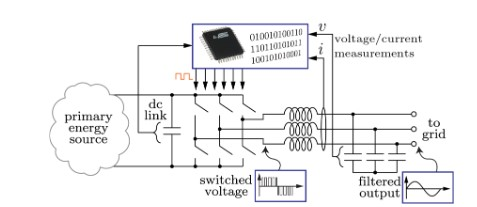
\includegraphics[scale=0.95]{images/chapter_2/Ch2F1.jpg}
% \caption{Grid Tied Source}
% \label{VPP sim}
% \end{figure*}


% Inverter-based DERs generally operate in either grid-following (GFL) or grid-forming (GFM) mode, with some hybrid or advanced modes combining features of both. A grid-following inverter behaves as a controlled current source that requires an external voltage reference (usually provided by the grid) to synchronize. It uses a phase-locked loop (PLL) to track grid voltage phase and frequency, and it injects current commands to deliver specified active and reactive power . By design, GFL inverters regulate their output current; during normal conditions they act like “voltage-controlled current sources” that adjust current based on grid conditions and control targets . In contrast, a grid-forming inverter controls its output as a voltage source, setting an internal reference for voltage magnitude and frequency (often with droop control) and can establish grid conditions in the absence of a strong external grid . GFM inverters can thus sustain an islanded microgrid by forming the reference voltage. Many GFM implementations emulate the dynamics of a synchronous machine – for example, via virtual synchronous machine (VSM) controls or droop characteristics – to provide inertia and damping. There are also hybrid control modes, such as “grid-supporting” inverters that use voltage- forming control but still synchronize to the grid, or inverters that can seamlessly switch between GFL and GFM mode (for instance, a BESS that operates grid-following when grid-connected and transitions to grid- forming during islanded operation ). Table 1 outlines key characteristics of different control schemes and their typical use in DER technologies.


% \begin{table}[htbp]
%     \centering
%     \begin{tabular}{|l|X|X|}
%     \hline
%     \textbf{Control Scheme}                & \textbf{Key Characteristics}                                                                                                                                          & \textbf{Typical DER Applications}                                           \\ \hline
%     Grid-Following (GFL)                   & \begin{tabular}[c]{@{}l@{}}- Relies on external voltage for synchronization (PLL-based)\\ - Limited fault current\\ - Cannot form islanded grid\end{tabular}            & \begin{tabular}[c]{@{}l@{}}- Solar PV\\ - Most battery inverters\\ - Type 4 wind turbines\end{tabular} \\ \hline
%     Grid-Forming (GFM)                     & \begin{tabular}[c]{@{}l@{}}- Can regulate voltage and frequency\\ - Capable of operating in islanded mode\\ - Better for stability and black-start\end{tabular}          & \begin{tabular}[c]{@{}l@{}}- Advanced battery inverters\\ - Some microgrids\\ - Future wind/PV systems\end{tabular} \\ \hline
%     Current-Controlled                     & \begin{tabular}[c]{@{}l@{}}- Regulates output current (e.g., for anti-islanding)\\ - May include current limiting\\ - Simplified response to faults\end{tabular}         & \begin{tabular}[c]{@{}l@{}}- Solar PV inverters\\ - Battery systems\end{tabular} \\ \hline
%     Voltage-Controlled                     & \begin{tabular}[c]{@{}l@{}}- Maintains voltage at terminals\\ - Can inject/absorb reactive power\\ - Supports voltage stability\end{tabular}                             & \begin{tabular}[c]{@{}l@{}}- Wind turbines with STATCOM functionality\\ - GFM inverters\end{tabular} \\ \hline
%     PQ Control                             & \begin{tabular}[c]{@{}l@{}}- Controls real (P) and reactive (Q) power output\\ - Often used with curtailment or export limits\end{tabular}                              & \begin{tabular}[c]{@{}l@{}}- Solar\\ - Aggregated DER fleets\end{tabular} \\ \hline
%     Droop Control                          & \begin{tabular}[c]{@{}l@{}}- Mimics governor/AVR behavior\\ - Enables decentralized coordination without communication\end{tabular}                                     & \begin{tabular}[c]{@{}l@{}}- Grid-forming DER\\ - Microgrids\\ - Hybrid systems\end{tabular} \\ \hline
%     Virtual Synchronous Machine (VSM)      & \begin{tabular}[c]{@{}l@{}}- Emulates inertia and damping of synchronous generators\\ - Enhances dynamic response\end{tabular}                                          & \begin{tabular}[c]{@{}l@{}}- High-performance BESS\\ - Research-stage DERs\end{tabular} \\ \hline
%     \end{tabular}
%     \caption{Overview of Control Schemes and Their Characteristics for DER Applications}
%     \label{tab:control_schemes}
% \end{table}

% \begin{figure*}[!h]
% \centering
% 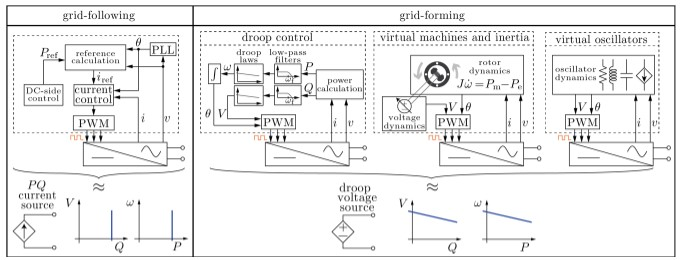
\includegraphics[scale=0.95]{images/chapter_2/Ch2F2.jpg}
% \caption{The comparison of  different control schemes}
% \label{VPP sim}
% \end{figure*}

% \subsection{IBR Terminal Voltage}

% The fault current contribution of an IBR is a function of its residual voltage (e.g., IBR terminal voltage or collector bus voltage during the fault) . However, the relationship between the inverter current and this residual voltage is nonlinear, which requires extensive testing or high-resolution transient simulation. Detailed IBR control system modeling is required to perform these simulations. Figure 2.12 and Figure 2.13 respectively show typical envelopes of maximum and minimum short-circuit currents as a function of residual voltage for Type IV wind turbine generators (with a full-scale back-to-back power converter as the interface with the grid) and Type III wind turbine generators (with doubly-fed asynchronous generator as the interface to the grid). Typically, voltage greater than 90\% is not considered a fault condition. When voltage is less than 20\%, most IBRs may cease operation (injection of current). As can be observed, the graphs are represented for different time frames after the fault. Similar curves can be obtained for any other type of IBR. 
% Another consideration in determination of the IBR residual terminal voltage is the interconnection transformer configuration. Typically, IBRs are interfaced with the host grid through an interconnection transformer that has at least one side in a delta configuration. This configuration will change the fault-induced voltage seen by the IBR measurement schemes installed on the IBR side of the interconnection transformer. Hence, a single-line-to-ground fault on the host grid can appear as a lesser voltage drop on two phases of the IBR terminal, which would reduce the IBR output current increase as  compared to a multi-phase fault. It is also important to note that the fault current contribution from the IBR is very minimal compared to the contribution of conventional synchronous machine based generating resources, which itself is a major challenge at high penetration levels.

% The terminal voltage of an IBR during a fault is a function of:

% Converter voltage reference $(v_{abc})$ generated by the control system,

% Filter and coupling impedance (L–R), and

% Grid voltage depression at the point of common coupling (PCC).

% In a simplified dq-frame model:
% % dq-axis terminal voltage of inverter
% \begin{equation}
% \label{eq:vtdq}
% \mathbf{V_{t,dq}} = \mathbf{V_{grid,dq}} + (R + j\omega L)\mathbf{I_{dq}}
% \end{equation}

% During a fault, the control algorithm regulates $I_d$ (active power component) and $I_q$ (reactive power component) according to LVRT and grid code requirements, resulting in a controlled but distorted terminal voltage waveform.


% \begin{figure*}[!h]
% \centering
% 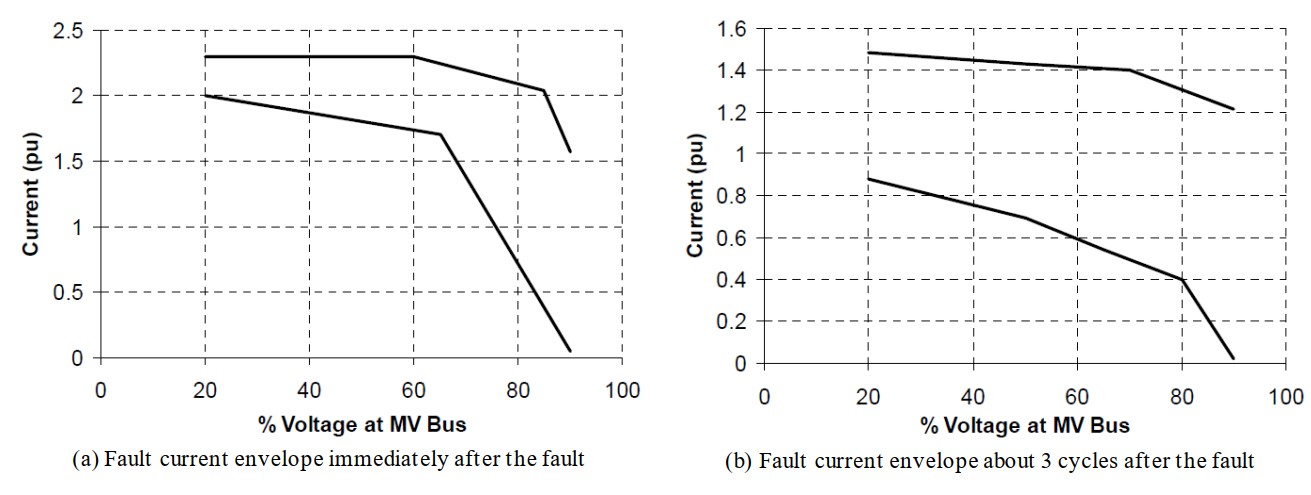
\includegraphics[scale=0.5]{images/chapter_2/Ch2F12Jul.jpg}
% \caption{Fault current levels for a Type IV wind turbine generator as a function of residual voltage at the point of common coupling}
% \label{VPP sim}
% \end{figure*}

% \begin{figure*}[!h]
% \centering
% 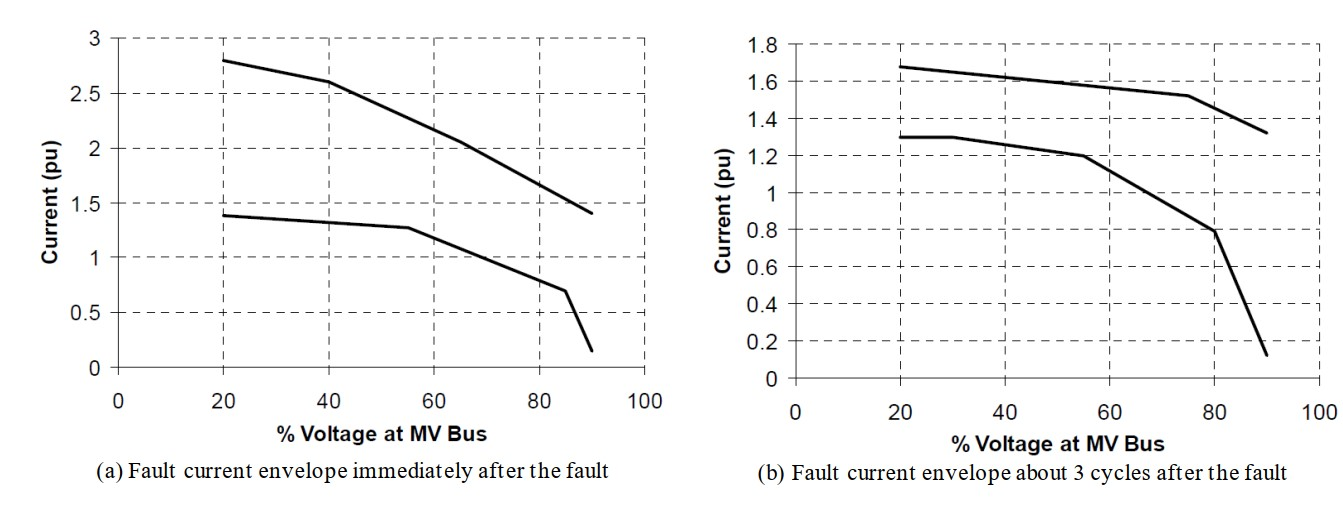
\includegraphics[scale=0.5]{images/chapter_2/Ch2F13Jul.jpg}
% \caption{Fault current levels for a Type III wind turbine generator with respect to IBR residual voltage }
% \label{VPP sim}
% \end{figure*}

% \subsection{Pre-Fault Operating Conditions}

% The IBR fault current contribution, particularly during the first few cycles following the fault, depends on the pre-fault operating conditions of the IBR, e.g., active and reactive power output levels, power factor, control set-points, pre-fault voltage, and input source condition (solar radiation, wind speed, etc.). Therefore, the analysis typically includes the full range of possible pre-fault operating conditions. However, since the search space of the operating conditions is quite large, a suitable approach is to calculate a maximum possible range of fault current. Generally, the magnitude of fault current contribution could vary from a minimum of zero to a maximum inverter current rating, depending on the pre-fault operating condition.

% Before fault initiation, the IBR operates under steady-state conditions delivering power as per its maximum power point tracking (MPPT) or set-point control. The inverter’s current reference maintains unity or near-unity power factor in GFL mode. This pre-fault condition defines the initial state of the control loops, influencing post-fault transients


% \subsection{Time Frame Following the Fault}

% The IBR fault response can be divided into three time frames:

% Sub-cycle (0–10 ms): Instantaneous voltage sag and current limiting due to DC-link dynamics.

% Converter control time (10–100 ms): PLL resynchronization and reactive current injection as per LVRT logic.

% Steady-state recovery (>100 ms): Gradual restoration of pre-fault operating point after fault clearance

% The fault current behavior of some IBRs that do not have a full-scale converter is relatively more complex than the IBRs with fully-rated converter (inverter) system. For example, in a Type III wind turbine generator, the nonlinearity of the crowbar system results in a complex fault behavior. The non-linear crowbar circuit is typically activated on severe faults or faults close to the generator. Upon activation, it shorts the rotor windings through a resistive circuit to protect them from overcurrents or damaging DC link overvoltages. 

% \subsection{Sequence Components of the Fault Current}

% During unbalanced faults, IBRs generate both positive- and negative-sequence currents depending on their control algorithms. The positive-sequence current supports voltage recovery, while negative-sequence current compensates unbalance. The zero-sequence component is typically absent unless a grounding path exists

% % The short-circuit analysis of conventional rotating-machine-based resources assumes that the performance of positive- and negative-sequence networks are fully decoupled, which is a fundamental assumption of symmetrical component analysis. The behavior of IBRs, however, is different from that of conventional rotating-machine-based resources as they usually attempt to maintain balanced current, even under unbalanced faults. 
% % The phase-angle of the fault current can be approximated based on the utility fault ride through requirements. Grid codes define reactive current injection as a function of residual voltage, but do not normally specify values for active current injection during faults. Thus, some assumptions are required to define the current phase-angle. The amplitude and angle of the fault current can also be specified by the manufacturer, if such level of detail is necessary for fault studies.

% \subsection{Power Electronic Transient Rating}


% Converter devices (IGBTs or SiC MOSFETs) possess limited overcurrent capability—typically 1.2–2.0 per unit for 1–2 cycles. Beyond this duration, overcurrent protection and control saturation mechanisms restrict further current increase to prevent semiconductor damage.

% % Most of the inverter manufacturers, particularly energy storage system vendors, provide both continuous and transient ratings for their products. Since the current contribution of the power electronic converter is in a typical range between 1.1 pu to 2.0 pu, the nominal and transient rating of the converter will determine the maximum fault current magnitude of the IBR. The transient overcurrent of the power converter allows higher fault capacity for adequate duration to support the protection system.

% \subsection{Power Electronic Protection}

% Protection functions include overcurrent, overvoltage, DC-link overcharge, and thermal monitoring. In case of severe faults, crowbar circuits (in DFIGs) or DC-link choppers (in PV inverters) bypass energy to protect the converter. Consequently, the IBR may temporarily disconnect or switch to reactive-only current mode.

% % There are typically conflicting requirements between the power electronic protection schemes and the utility low voltage fault ride through requirements. For distribution interconnections, the utility requires the IBR to disconnect from the electric grid within a specified period of time after occurrence of a fault . Therefore, the IBR protection can affect the level and time frame of the IBR currents when a fault occurs. In addition, the power electronic protection elements may qualify a system fault and disconnect (or block the currents) because of incorrect frequency measurement and/or sensitivity to harmonics induced by the fault, particularly in weak systems. Thus, evaluating frequency protection elements for the power electronic devices as a part of protection studies is valuable.
% \section{Network configurations and system parameters}


% \section{Modelling Grid Tied PV sources}
% % Structure of generic positive sequence grid forming model to capture structural and operational similarity across four different grid forming methods




% \begin{figure*}[!h]
% \centering
% 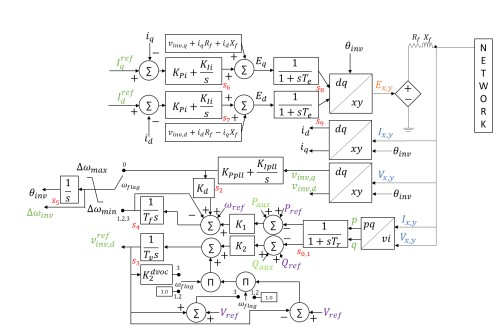
\includegraphics[scale=1.2]{images/chapter_2/Ch2F8.jpg}
% \caption{ Structure of generic positive sequence grid forming model to capture structural and operational similarity across four different grid forming methods}
% \label{VPP sim}
% \end{figure*}

% \begin{figure*}[!h]
% \centering
% 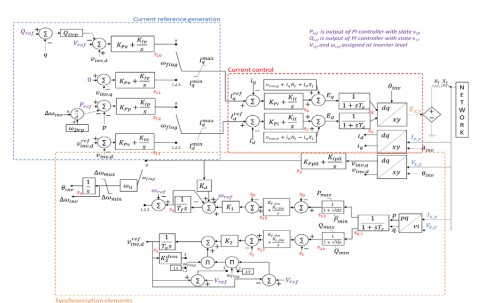
\includegraphics[scale=1.2]{images/chapter_2/Ch2F9.jpg}
% \caption{Generic grid forming (GFM) renewable generator/converter model}
% \label{VPP sim}
% \end{figure*}


% \begin{figure*}[!h]
% \centering
% 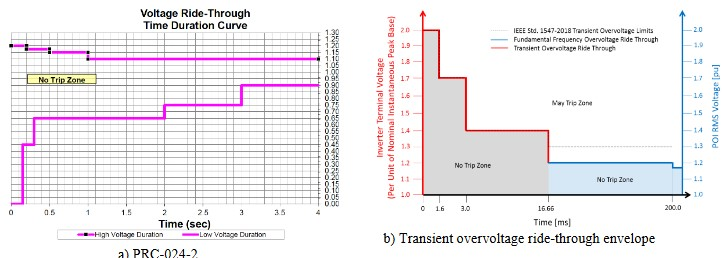
\includegraphics[scale=0.95]{images/chapter_2/Ch2F3.jpg}
% \caption{LVRT requirements}
% \label{VPP sim}
% \end{figure*}


% \subsection{Grid Code Requirements}



% % Figure 2.4 shows an example of transmission interconnection of two inverter-based generating stations to the integrated power system. The solar generating station is interconnected to the grid through a line that already has a tapped transmission customer, whereas the wind turbine generating station is interconnected through a dedicated line. Two conventional generating stations (CG1 and CG2) within the integrated power system are comprised of synchronous sources whose size and short circuit strength are significantly more than either of the inverter-based generating stations. 

% Grid codes (IEEE 1547-2018, IEC 61400-21, ENTSO-E) mandate that DERs remain connected during short voltage dips (fault ride-through). The requirements typically include:

% Voltage–time LVRT profile defining mandatory connection zones.

% Reactive current injection proportional to voltage deviation.

% Frequency ride-through for sustained operation during frequency excursions.

% Each grid code differs in detail—for instance, European standards emphasize reactive current support, while North American codes specify both positive- and negative-sequence current behavior.


% \begin{figure*}[!h]
% \centering
% 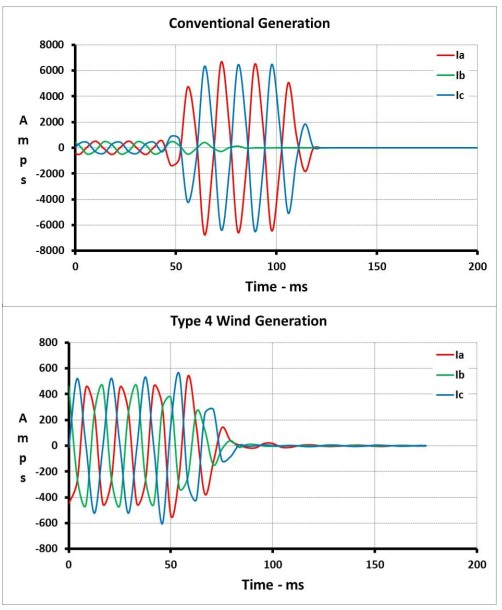
\includegraphics[scale=0.95]{images/chapter_2/Ch2F5Jul.jpg}
% \caption{ Dissimilar short circuit responses of conventional generation and Type IV 
% wind turbine facilities to a phase-to-phase fault}
% \label{VPP sim}
% \end{figure*}


% % The following example was an internal phase-to-phase fault (A-to-C) on a short 138 kV line interconnecting a 100 MW Type IV wind turbine facility to the grid. The interconnection configuration was similar to Figure 2.4 where the wind turbine facility was connected by the line between CB2 (Circuit Breaker 2) and CB4 (Circuit Breaker 4). Figure 5 shows the short circuit current waveforms captured by the line protection relays.The example presented illustrates the significantly different short circuit response of an  IBR compared to the integrated system or cluster of interconnected conventional synchronous sources. 



% \subsubsection{Fault ride through}
% % As the size of IBR facilities started to increase and their installed capacity within a transmission system began to rise, transmission planners started to recognize system integration challenges. Utilities and the regulators around the world in-turn introduced grid codes with additional requirements to connect the IBR facilities. These interconnection requirements influenced control system designs of the IBRs, thereby their short circuit current outputs and consequently protection responses. Most utilities or utility regulators now have their own interconnection requirements. Using the German grid code as an example, this section introduces and illustrates the relevance of the code to the line protection systems with IBR facilities.

% The Fault Ride-Through (FRT) capability ensures DERs support the grid during transient faults without tripping. FRT algorithms maintain converter operation through reactive current support and DC-link management.


% \subsubsection{IBR Low Voltage Ride Through}

% % According to this requirement, the source is to remain connected when the voltage depression from an external fault is within the low-voltage ride-through requirement of the applicable grid code. Due to this requirement, the short-circuit current characteristics of the IBRs have become relevant to the line protection security. An undesirable line protection operation during an external short circuit will disconnect the generator and defeat requirements specified by the grid code.

% When voltage drops below a threshold (e.g., 0.9 p.u.), LVRT logic triggers reactive current injection:
% % LVRT reactive current injection rule
% \begin{equation}
% \label{eq:lvrt}
% I_q = K_q (V_{ref} - V_{pcc})
% \end{equation}

% where (K) defines the slope of current-voltage characteristic. DFIG systems use rotor converters to control stator voltage, whereas full converters regulate grid-side current directly.

% \begin{figure*}[!h]
% \centering
% 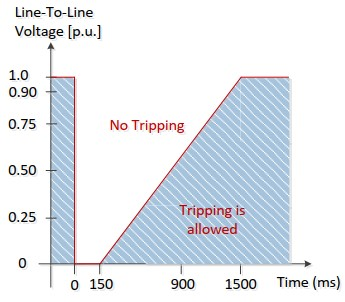
\includegraphics[scale=0.95]{images/chapter_2/Ch2F6Jul.jpg}
% \caption{Low voltage ride through requirement by the German grid code}
% \label{VPP sim}
% \end{figure*}


% \subsubsection{IBR Positive Sequence Reactive Current Injection}

% IBRs inject positive-sequence reactive current in phase opposition to voltage depression, thereby supporting grid voltage restoration. This current is limited by converter rating and grid code-defined proportionality constants.

% % In case of voltage  depression, the source is required to supply positive sequence reactive current, irrespective of fault type. This increased reactive current is required to minimize voltage depression during faults and assist in preventing loads such as induction motors from stalling and further depressing the voltage. Similarly, the source is required to absorb positive sequence reactive current during overvoltage conditions, to thereby help in returning the voltage to 
% % a normal level.

% \begin{figure*}[!h]
% \centering
% 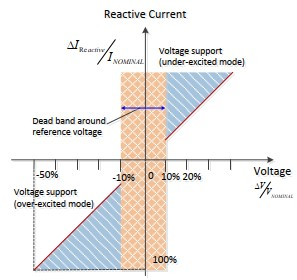
\includegraphics[scale=0.95]{images/chapter_2/Ch2F7Jul.jpg}
% \caption{Positive sequence dynamic reactive current requirements during voltage excursions}
% \label{VPP sim}
% \end{figure*}


% \subsubsection{IBR Negative Sequence Reactive Current Injection}

% To mitigate voltage unbalance, converters may inject negative-sequence current at controlled amplitude and phase, ensuring symmetrical voltage recovery and minimizing torque oscillations in rotating machines.

% % Negative sequence relaying became easily available after the introduction of multifunction microprocessor-based relays in the marketplace. Because of benefits such as negative sequence elements being unaffected by zero sequence mutual coupling and improved sensitivity to high resistance ground faults, utilities started to widely apply negative sequence relaying in transmission line protection applications for unbalanced faults, 
% % particularly for the ground faults. Except for one recently introduced new grid code VDE-AR-N 4130 in Germany, none of the other utilities (at the time of this writing) has a requirement concerning negative sequence current injection. Hence, the IBR manufacturers typically in their present day control system designs supress negative sequence current. Absence of adequate negative sequence current during unbalanced faults, as a consequence, is threatening protection reliability i.e. its ability to adequately protect the line during unbalanced faults.

% \begin{figure*}[!h]
% \centering
% 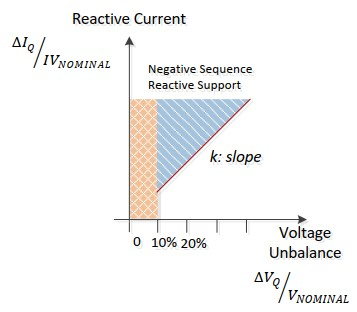
\includegraphics[scale=0.95]{images/chapter_2/Ch2F8Jul.jpg}
% \caption{Requirement for negative sequence reactive current injection 
% proportional to negative voltage unbalance }
% \label{VPP sim}
% \end{figure*}


% \subsubsection{IBR Zero Sequence Reactive Current Injection}

% Zero-sequence current control is generally suppressed to avoid DC-link oscillations and ground fault overcurrents unless a dedicated grounding transformer is available.

% Power electronic sources are typically not grounded so no zero sequence current injection requirements exist. In this regard the IBR is no different than the typical utility-connected conventional generator which is supplies only small zero sequence current.

% \subsubsection{IBR Frequency Ride Through}

% Nearly all regional transmission regulators and transmission utilities have frequency ride through requirements for interconnecting generators. Figure 10, taken from NERC PRC-024-1 , illustrates ride through requirements from different North American regional entities. These requirements apply to all types of generators, conventional sources and IBR, facilities, with the exception in Quebec, Canada where they allow IBRs (asynchronous resources such as photovoltaic and wind turbine generators) to trip instantaneously above 61.7 Hz instead of 66 Hz.  
% Frequency ride-through (FRT) ensures DER continuity under frequency deviations. Active power modulation is executed via droop control or virtual inertia algorithms, avoiding premature disconnection.

% \begin{figure*}[!h]
% \centering
% 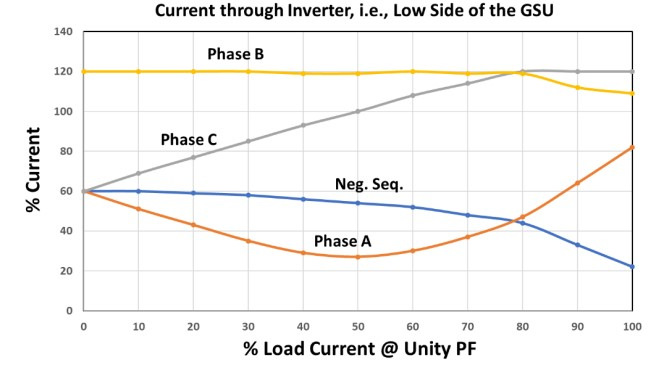
\includegraphics[scale=0.95]{images/chapter_2/Ch2F9Jul.jpg}
% \caption{Estimation of current through inverter for close-in (on high-side of unit 
% transformer) line-to-line fault }
% \label{VPP sim}
% \end{figure*}

% \begin{figure*}[!h]
% \centering
% 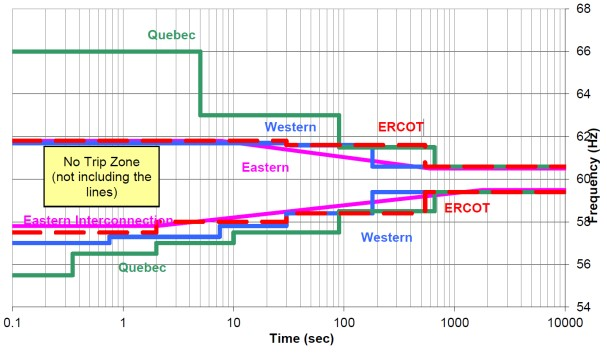
\includegraphics[scale=0.95]{images/chapter_2/Ch2F10Jul.jpg}
% \caption{Frequency ride through requirements of North American regional entities}
% \label{VPP sim}
% \end{figure*}





% \section{IBR Response to network faults}

% % To properly evaluate the impact of IBR on the protection system, it is essential to obtain an accurate understanding of the fault current characteristics and contribution levels of various types of IBR. The fault response of an IBR is fundamentally determined by the control strategy of its power-electronic converter or inverter system, which varies among different manufacturers.  In general, most IBRs are controlled for constant-power output with current limiting functionality, which act as current sources. 

% % In most existing designs with full converter interface, the IBR only injects positive sequence current under all operating conditions including balanced and unbalanced faults. This is referred to as coupled sequence control (CSC) scheme. This means that there will not be any negative sequence fault current from the IBR during an unbalanced network fault. Lack of negative sequence current contribution poses a big challenge to traditional protection schemes in transmission systems . 

% The IBR’s fault current is limited, controllable, and transiently reactive. Without grid codes, the inverter ceases injection upon voltage drop. With grid codes enforced, reactive current support modifies the current phase angle, producing dynamic apparent impedance trajectories that challenge traditional relays.

% \begin{figure*}[!h]
% \centering
% 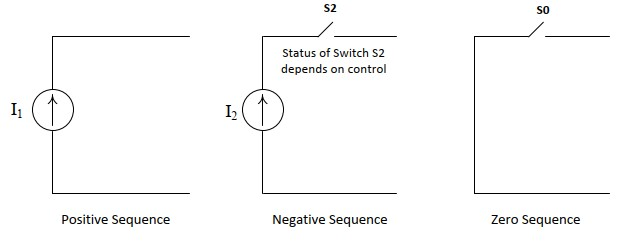
\includegraphics[scale=0.95]{images/chapter_2/Ch2F11Jul.jpg}
% \caption{A simplified positive-, negative- and zero-sequence equivalent of an IBR}
% \label{VPP sim}
% \end{figure*}

% \subsection{Without codes}
% Earlier inverters disconnected instantly under undervoltage, causing loss of generation and system instability. Protection schemes relying on fault current magnitudes often failed to detect faults near the DER terminal.
% \subsection{With grid codes}
% Modern IBRs remain connected during LVRT events, injecting reactive current within 20–40 ms, changing the fault current waveform. This controlled behavior requires new directional and impedance-based protection philosophies.
% \subsection{Summary of DER Interconnection Requirements in IEEE 1547}
% IEEE 1547-2018 defines:

% Reactive power priority during LVRT,

% Frequency ride-through between 56–62 Hz,

% Communication-based coordination using IEEE 2030.5 or Modbus,

% Clear criteria for reconnection post-fault.
% \subsection{Characteristics of DER for Protection}

% Fault current: 1.1–1.3 p.u.

% Dominant reactive content.

% Controlled phase shift relative to pre-fault voltage.

% Asymmetric sequence contributions under unbalanced faults.

% These characteristics render current-magnitude-based relays unreliable.











